\subsection{Montel 空间}

定义 4. --- 每个有界子集都相对紧的局部凸 Hausdorff 桶型空间称为 Montel 空间。

例. --- 1) 每个有限维 Hausdorff 空间都是 Montel 空间。是 Montel 空间的赋范空间是局部紧的，从而是有限维的（I，第 15 页，定理 3）。

\begin{enumerate}
\def\labelenumi{\arabic{enumi})}
\setcounter{enumi}{1}
\tightlist
\item
  采用 III 第 6 页的命题 7 的记号与假设，空间 E 作为 Banach 空间的归纳极限是桶型的（III，第 25 页）；此外，E 的每个有界子集都相对紧（III，第 6 页，命题 7）。换言之，E 是一个 Montel 空间。
\end{enumerate}

特别地，Gevrey 空间（III，第 10 页）是 Montel 空间。* 这对空间 \(\mathcal{H}(\mathbf{K})\) 也成立，它由在紧子集 \(\mathbf{K}\)（\(\mathbf{C}^n\) 的）的一个邻域中解析的函数的芽组成（III，第 10 页）。*

\begin{enumerate}
\def\labelenumi{\arabic{enumi})}
\setcounter{enumi}{2}
\tightlist
\item
  Montel 空间序列 \((\mathrm{E}_{n})\)（II，第 33 页）的每个严格归纳极限 E（使得对所有 n，\(E_{n}\) 在 \(E_{n+1}\) 中闭）都是 Montel 空间；事实上，E 是 Hausdorff 的（II，第 32 页，命题 9 (i)）、桶型的（III，第 25 页，推论 3），且 E 的每个有界子集都包含在某个 \(E_{n}\) 中（III，第 5 页，命题 6），从而在 \(E_{n}\) 中相对紧，因而在 E 中也相对紧。
\end{enumerate}

* 4) 设 U 是 \(\mathbf{R}^n\) 中的一个开集，\(\mathcal{C}^\infty (\mathrm{U})\) 是 U 上无穷次可微函数组成的 Fréchet 空间（III，第 9 页）。我们将证明它是一个 Montel 空间。由于 \(\mathcal{C}^\infty (\mathrm{U})\) 是 Fréchet 空间，它是桶型的（III，第 25 页，推论）。设 B 是 \(\mathcal{C}^\infty (\mathrm{U})\) 的一个有界子集，K 是 U 的一个紧子集。对每个 \(\alpha \in \mathbf{N}^n\)，设 \(\mathrm{H}_{\alpha ,\mathrm{K}}\) 是函数 \(\partial^{\alpha}f\)（\(f\) 取遍 B）在 K 上的限制组成的集。设 \(\alpha \in \mathbf{N}^n\)；对每个 \(\beta \in \mathbf{N}^n\)（满足 \(|\beta | = |\alpha | + 1\)），集 \(\mathrm{H}_{\alpha ,\mathrm{K}}\) 在 \(\mathcal{C}(\mathbf{K})\) 中有界，因为 B 在 \(\mathcal{C}^\infty (\mathrm{U})\) 中有界；由 VAR, R., 第 2.2.3 目，集 \(\mathrm{H}_{\alpha ,\mathrm{K}}\) 是等度连续的，故（GT，X，§ 2，第 5 目）

在 \(\mathcal{C}(\mathbf{K})\) 中相对紧。而 \(\mathcal{C}^{\infty}(\mathbf{U})\) 的拓扑是使所有映射 \(f\mapsto \partial^{\alpha}f|\mathbf{K}\)（从 \(\mathcal{C}^{\infty}(\mathbf{U})\) 到 \(\mathcal{C}(\mathbf{K})\) 中的）连续的拓扑中最粗的，因此 \(\mathbf{B}\) 在 \(\mathcal{C}^{\infty}(\mathbf{U})\) 中相对紧（GT，I，§ 4，第 1 目，命题 3 与 § 9，第 5 目，推论）。

类似地，U 中具有紧支集的无穷次可微函数全体组成的空间 \(\mathcal{C}_0^\infty (\mathrm{U})\)（III，第 9 页）是 Montel 空间。因为 \(\mathcal{C}_0^\infty (\mathrm{U})\) 是 Fréchet 空间序列 \(\mathcal{C}_{\mathrm{H}_n}^\infty (\mathrm{U})\) 的严格归纳极限（III，第 9 页），而只需看出每个空间 \(\mathcal{C}_{\mathrm{H}_n}^\infty (\mathrm{U})\) 都是 Montel 空间（例 3）。但 \(\mathcal{C}_{\mathrm{H}_n}^\infty (\mathrm{U})\) 的有界闭子集在 \(\mathcal{C}^{\infty}(\mathrm{U})\) 中闭且有界，从而在 \(\mathcal{C}^{\infty}(\mathrm{U})\) 中紧，因而在 \(\mathcal{C}_{\mathrm{H}_n}^\infty (\mathrm{U})\) 中也紧。

命题 8. --- 设 E 是一个 Montel 空间，F 是 E 上的一个滤子，它对于弱化拓扑收敛于 E 中的点 \(x_{0}\)。若 F 具有可数基，或包含一个有界集，则 F 也对于初始拓扑收敛于 \(x_{0}\)。

先假定 F 中存在一个有界集 B。B 对于 E 的初始拓扑的闭包 \(\overline{B}\) 是有界的；此外，\(\overline{B}\) 是紧的，因为 E 是 Montel 空间。\(\overline{B}\) 上由 \(\sigma(E, E')\) 诱导的拓扑是 Hausdorff 的，且比由初始拓扑诱导的拓扑粗；因此二者一致（GT，I，§ 9，第 4 目）。这就证明了此情形下的命题。

其次假定 \(\mathfrak{F}\) 具有可数基。只需（GT，I，§6，第 8 目，命题 11）考虑序列 \((x_{n})_{n\geqslant 1}\) 收敛于 \(x_0\)（对于 \(\sigma (\mathrm{E},\mathrm{E}^{\prime})\)）的情形。设 B 是所有 \(x_{n}\)（\(n\geqslant 0\)）组成的集。这个集对于 \(\sigma (\mathrm{E},\mathrm{E}^{\prime})\) 有界，从而对于初始拓扑也有界（III，第 27 页，推论 3）。于是我们已归结为证明的第一种情形。

每个 Montel 空间都是自反的：这由定义 4 与 IV 第 16 页的定理 2 得出。此外：

命题 9. --- Montel 空间的强对偶是 Montel 空间。

设 E 是一个 Montel 空间，\(E_{b}^{\prime}\) 是它的强对偶。由于 E 是自反的，\(E_{b}^{\prime}\) 是桶型的（IV，第 15 页，定理 1）。由于 E 的每个有界子集都相对紧，\(E^{\prime}\) 上的强拓扑与紧收敛拓扑一致。设 B 是 \(E_{b}^{\prime}\) 的一个有界子集；它对于弱拓扑 \(\sigma(E^{\prime}, E)\) 有界，从而是等度连续的，因为 E 是桶型的。于是 Ascoli 定理（GT，X，§ 2，第 4 目，推论与 § 2，第 5 目，推论 1）蕴含 B 对于 \(\sigma(E^{\prime}, E)\) 的闭包对于紧收敛拓扑是紧的；因此 B 在 \(E_{b}^{\prime}\) 中相对紧。

命题 10. --- 每个可度量化 Montel 空间都满足第一可数公理。

设 E 是一个可度量化 Montel 空间。我们知道（II，第 5 页），E 可以等同于赋范空间序列的乘积 \(F = \prod_{n \in N} F_n\) 的一个子空间，甚至可以假定 \(\Pr_n(E) = F_n\)（对所有 \(n \in N\)）。若每个可度量化空间 \(F_n\) 都满足第一可数公理，则 F 也满足（GT，IX，§ 2，第 8 目），从而 E 也满足。

我们用反证法论证。例如假定 \(F_{0}\) 不满足第一可数公理。设 \(B_{0}\) 是 \(F_{0}\) 中的（闭）单位球；这是一个不满足第一可数公理的度量空间。我们将使用下列引理：

引理 1. --- 设度量空间 X 不满足第一可数公理。则存在实数 \(\varepsilon > 0\) 与 X 中的不可数子集 A，使得 \(d(x, y) \geqslant \varepsilon\)（对 A 中所有不同的 \(x, y\)）。

对每个整数 \(n \geqslant 1\)，设 \(\mathfrak{F}_n\) 是由这样的子集 \(D\)（\(X\) 的）组成的集（按包含关系排序）：\(d(x, y) \geqslant \frac{1}{n}\)（对不同的 \(x, y\)，属于 \(D\)）。集 \(\mathfrak{F}_n\) 具有有限特征，从而具有一个极大元素 \(D_n(S, III, \S 4, No. 5)\)。于是对所有 \(y \in X\)，存在点 \(x\)（\(D_n\) 中的）使得 \(d(x, y) < \frac{1}{n}\)，这由 \(D_n\) 的极大性得出。令 \(D = \bigcup_{n} D_n\)；则集 \(D\) 在 \(X\) 中稠密，且由于 \(X\) 不满足第一可数公理，\(D\) 不是可数的，从而某个 \(D_n\) 不是可数的。

证毕。

把引理 1 应用于 \(\mathbf{B}_0\)，存在不可数子集 \(\mathbf{A}_0\)（\(\mathbf{F}_0\) 中的）以及一个数 \(\varepsilon > 0\)，使得 \(\| x \| \leqslant 1\) 且 \(\| x - y \| \geqslant \varepsilon\)（对不同的 \(x, y\)，属于 \(\mathbf{A}_0\)）。我们有 \(\mathrm{pr}_0(\mathrm{E}) = \mathrm{F}_0\)，因而存在子集 \(\mathbf{A}\)（\(\mathbf{E}\) 中的），使得 \(\mathrm{pr}_0\) 诱导一个从 \(\mathbf{A}\) 到 \(\mathbf{A}_0\) 上的双射。

引理 2. --- 存在一个由 A 中不同元素组成的序列 \((x_{m})_{m\geqslant 0}\)，它在 E 中有界。

我们将用归纳法构造 A 的点的一个序列 \((x_{m})_{m\geqslant 0}\)，以及 A 的子集的一个递减序列 \((\mathrm{C}_m)_{m\geqslant 0}\)，它们满足下列条件：

\begin{enumerate}
\def\labelenumi{\alph{enumi})}
\item
  每个集 \(\mathbf{C}_m\) 都不是可数的。
\item
  对每个 \(n \geqslant 0\)，集 \(\mathrm{pr}_k(\mathbf{C}_m)\) 在 \(\mathbf{F}_k\) 中有界（对 \(0 \leqslant k \leqslant m\)）。
\item
  对每个 \(m \geqslant 0\)，我们有 \(x_{m} \in \mathbf{C}_{m} - \mathbf{C}_{m+1}\)。
\end{enumerate}

令 \(C_0 = A\)。假定诸集 \(C_m\)（对 \(0 \leqslant m \leqslant n\)）已定义，使得 a) 与 b) 对 \(0 \leqslant m \leqslant n\) 满足，且点 \(x_m\)（在 \(C_m - C_{m+1}\) 中的，对 \(0 \leqslant m < n\)）也已定义。对每个整数 \(r \geqslant 1\)，设 \(C_{n,r}\) 是所有满足下列条件的 \(x \in C_n\) 组成的集：

\[
r - 1 \leqslant \left\| \operatorname{pr} _ {n + 1} (x) \right\| <   r.
\]

由于 \(\mathbf{C}_n\) 不是可数的，存在整数 \(r \geqslant 1\) 使得 \(\mathbf{C}_{n,r}\) 不是可数的。我们选取一点 \(x_n\)（在 \(\mathbf{C}_{n,r}\) 中），并令 \(\mathbf{C}_{n+1} = \mathbf{C}_{n,r} - \{x_n\}\)。显然 \(\mathbf{C}_{n+1} \subset \mathbf{C}_n\) 且 \(x_n \in \mathbf{C}_n - \mathbf{C}_{n+1}\)，集 \(\mathbf{C}_{n+1}\) 不是可数的，且 \(\mathrm{pr}_k(\mathbf{C}_{n+1})\) 在 \(\mathbf{F}_n\) 中有界（对 \(0 \leqslant k \leqslant n + 1\)）。

我们有 \(x_{m} \in C_{m}\)，从而 \(x_{m} \in C_{n}\)（当 \(m \geqslant n\) 时）。因此序列 \((x_{m})_{m \geqslant 0}\) 在 \(F_{n}\) 上的投影对所有 \(n \geqslant 0\) 有界；换言之，序列 \((x_{m})_{m \geqslant 0}\) 在 E 中有界，这就证明了引理 2。

证毕。

采用引理 2 的记号，有界序列 \((x_{m})_{m\geqslant 0}\) 在 E 中有一个极限点 \(y\)。于是序列 \((\mathrm{pr}_0(x_m))_{m\geqslant 0}\) 有一个极限点 \(\mathrm{pr}_0(y)\)（在 \(\mathbf{F}_0\) 中），但这与 \(\mathbf{A}_0\) 的构造矛盾。

推论. --- 设 E 是一个可度量化 Montel 空间。则 E 的强对偶中存在一个可数稠密集。

在 E 的对偶 \(E'\) 上，强拓扑与紧收敛拓扑相同，因为 E 是 Montel 空间。于是只需应用 III 第 18 页的命题 6 的推论 1。

\pandocbounded{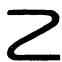
\includegraphics[keepaspectratio]{images/part002_3e739bde.jpg}}

我们可以证明，可度量化 Montel 空间 \(E\) 的强对偶当 \(E\) 是无限维时不是可度量化的（IV，第 57 页，习题 1）。

